\documentclass{article}
\title{CSCI 2200 HW1}
\author{Xinshi,Wang}
\usepackage[letterpaper,textwidth=5.5in,right=0.6in,textheight=9in,left=0.6in,top=0.7in,bottom=0.7in]{geometry}
\usepackage{scrextend}
\usepackage{graphicx}
\usepackage{xcolor}
\usepackage{amssymb}
\usepackage{amsmath}
\usepackage{setspace}
\usepackage{mathrsfs}
\usepackage[utf8]{inputenc}
\usepackage{mathtools}
\begin{document}
\noindent
CSCI 2200 HW3\\
Wang Xinshi\\

%Q 12.8 starts from here
\begin{addmargin}[2em]{2em}
	\text{\bf Problem 15.15} Among 400 students, 150 are in math, 120 are in bio and 50 are math-bio duals. What are the chances a random student is in: (a) math or bio (b) bio and not math (c) neither math nor bio?\\
	
	\noindent (a)$\left |Math \cup Bio \right| = \left |Math \right| + \left |Bio \right| - \left |Math \cap Bio \right|$.

	Thus
	\begin{align*}
		P(\left |Math \cup Bio \right|) &= P(\left |Math \right|) + P(\left |Bio \right|) - P(\left |Math \cap Bio \right|)\\
		&= \dfrac{150}{400}+\dfrac{120}{400}-\dfrac{50}{400}\\
		&= \dfrac{11}{20}
	\end{align*} 

	\noindent (b)$\left |Math^c \cap Bio-Math \right| = \left |Bio-Bio \ capMath \right|$, since biology is a subset of not math.
		
	Thus
	\begin{align*}
		P(\left |Math^c \cap Bio \right|) &= P(\left |Bio - Bio \cap Math \right|)\\
		&= \dfrac{70}{400}\\
		&= \dfrac{7}{40}
	\end{align*} 

	\noindent (c)$\left |Math \cup Bio \right|^c = \Omega - \left |Math \cup Bio \right|^c$.
	
	Thus
	\begin{align*}
		P(\left |Math \cup Bio \right|^c) &= P(\Omega) - P(\left |Math \cup Bio \right|^c|)\\
		&= 1 - \dfrac{11}{20}\\
		&= \dfrac{9}{20}
	\end{align*} 
\end{addmargin}
%Q 12.8 ends here 

\clearpage

%Q 11.13 starts from here
\begin{addmargin}[2em]{2em}
	\text{\bf Problem 16.37}.There are two beavers, brown and black. What are the chances both are male? What if you know:
	(a) one is male (b) one is male and one is born on a Tuesday (c) one is a male born on a Tuesday?
	Verify answers with Monte Carlo simulation. How strange, the birthday of a beaver changes the probability of two males.\\
	
	(a)
	The sample space is $\{MM,MF,FM\}$
	\begin{align*}
		P[\text{Both are male}|\text{One is Male}] = \dfrac{1}{3}.\\
	\end{align*}

	(b).
	The sample space is $\{MM2,MF2,F2M\}$.
	\begin{align*}
		P[\text{Both are Male}|\text{One is Male and One is born on Tuesday}] = \dfrac{1}{3}.\\
	\end{align*}

	(c).
	The sample space is $\{M1M2,M2M2....,M2M1,....\}$.
	\begin{align*}
		P[\text{Both are Male}|\text{One is Male and One is born on Tuesday}] = \dfrac{13}{27}.\\
	\end{align*}
\end{addmargin}

%Q 11.13 ends here

\clearpage

%Q 11.71(a) starts from here
\begin{addmargin}[2em]{2em}
	\text{\bf Problem 16.42}. Five out of $100$ coins are two-headed. You randomly pick a coin and flip it “fairly” twice (each side
	is equally probable). What is the probability to get (a) $2$ heads (b) $2$ tails (c) matching tosses?
	
	\begin{figure}[ht]
		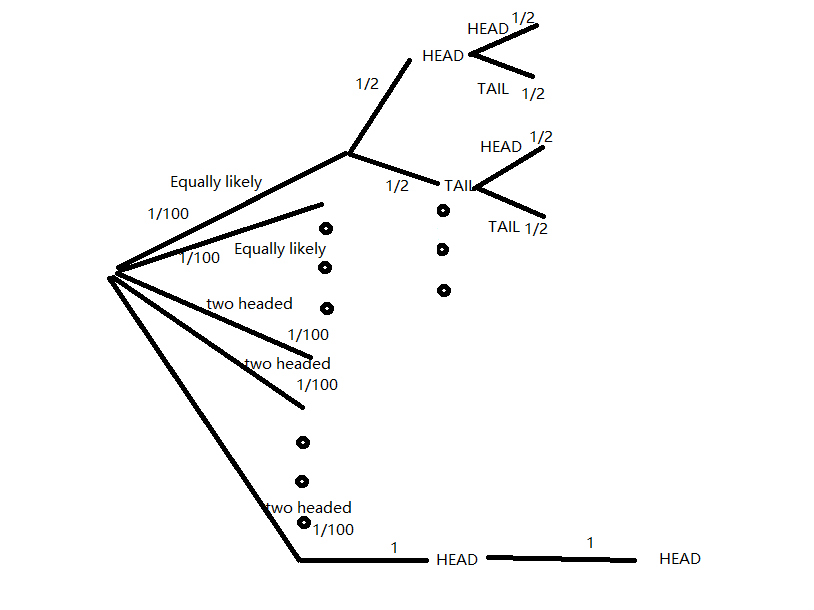
\includegraphics[scale = 0.3]{"C:/Users/Micha/OneDrive - Rensselaer Polytechnic Institute/CSCI 2200/Latex_pictures/PROB-TREE.png"}
	\end{figure}
	(a). According to the probabability tree, we have $P(\text{2 heads}) = \sum_{i=1}^{95} \dfrac{1}{400} + \sum_{i=96}^{100} \dfrac{1}{100} = \dfrac{95}{400}+\dfrac{5}{100} = \dfrac{23}{80}$.\\
	
	(b). According to the probabability tree, we have $P(\text{2 tails}) = \sum_{i=1}^{95} \dfrac{1}{400} + \sum_{i=96}^{100} 0 = \dfrac{95}{400} =  \dfrac{19}{80}$.\\
	
	(c). According to the probabability tree, we have $P(\text{2 tosses match}) = \sum_{i=1}^{95} \dfrac{2}{400} + \sum_{i=96}^{100} \dfrac{1}{100} = \dfrac{90}{400}+\dfrac{5}{100} = \dfrac{21}{40}$.
\end{addmargin}
%Q 11.71(a) ends here

\clearpage
%Q 12.31 starts from here
\begin{addmargin}[2em]{2em}
\text{\bf Problem 16.81.}You have a fair $5$-sided die which can generate one of the numbers $\{1, 2, 3, 4, 5\}$ with probability
$\dfrac{1}{5}$ each. You wish to simulate a fair $7$-sided die which generates a number in $\{1, 2, 3, 4, 5, 6, 7\}$ with probability $\dfrac{1}{7}$
each. Give an algorithm to do so, and prove it.\\

Toss a coint 2 twice, $\forall (i,j) \in \{1...5\}\times\{1...5\}$, we have $(1,1)=1,(2,2)=2,(3,3)=3,(4,4)=4,(5,5)=5,(5,1)=6,(5,2)=7$. Other wise, we restart.\\

Prove: Let $n$ be an arbitrary number and $n \in \{1,..,7\}$. We have 
\begin{align*}
	P[n]&=p[n|(1,1)]P[(1,1)]+p[n|(1,2)]P[(1,2)]+...+p[n|(i,j)]P[(i,j)]+P[n|restart]P[restart]\\
	P[n]&=\dfrac{1}{25}(\text{since there will be only 1 exact match}) + \dfrac{18}{25}P[n]\\
	\dfrac{17}{25}P[n]&=\dfrac{1}{25}\\
	P[n] &= \dfrac{1}{7}\\
\end{align*}
\end{addmargin}
%Q 12.31 ends here

\clearpage

%Q 12.74(k) starts from here
\begin{addmargin}[2em]{2em}
\text{\bf Problem 17.35}. You have 100 and bet 1 at a time on roulette. You goal is to win 50. Compute the probability that you reach your goal before going bankrupt.\\

I here assume it is exactly the same roulette as the one on the book.

probability of landing on red (probability of winning) = $\dfrac{18}{38}$. There are fifty steps away from winning, thus $L=150$.
The formula is $P(k,l,p) = \dfrac{p^k-p^l}{p^k-1}$.\\
Thus we have $P[win] = P(50,150,p) = \dfrac{0.9^{150}-0.9^{50}}{0.9^{150}-1} = 2.64 \times 10^-5$.
\end{addmargin}
%Q 12.74(k) ends here
\newpage
%Q 12.74(k) starts from here
\begin{addmargin}[2em]{2em}
	\text{\bf Problem 18.59}. For 20 fair coin flips, define events A = $\{\text{equal number of H and T}\}$ and B = $\{\text{first 3 flips are H}\}$.
	Compute the probabilities: (a) A occurs. (b) B occurs. (c) A and B occur. (d) A or B occur.\\
	
	(a). We are choosing 10 from 20
	$P[A] = \dfrac{\binom{20}{10}}{2^20} = \dfrac{183746}{20^20} = 0.17$.\\
	
	(b). $P[B] = \dfrac{1}{2^3} = \dfrac{1}{8}$.\\
	
	(c). $P[A \cap B] = P[A] \times  \binom{17}{7} \times 0.5^7 \times 0.5^{10} = 0.125 \times 0.148 = 0.0185$\\
	
	(d)$P[A \cup B] = P[A]+P[B]-P[A \cap B] = 0.283$.
	
\end{addmargin}
%Q 12.74(k) ends here
\end{document}